\chapter[Implementering af software]{Software}

% Note om hvad der skal stå i dette afsnit her.


\section{Oversigt over softwaren}

% Her skriver vi hvordan softwaren er struktureret - se figuren nedenfor.

Softwaren er struktureret som vist i
figur\vref{fig:software-oversigt}. Dataføderen leverer data til den
del af softwaren, der behandler HPGL. Dataen kommer fra et
SD-kort. HPGL-behandleren sender instruktioner videre til den del af
motorkontrollen, der afvikles når der er tid. Denne del sætter
instruktioner i kø til realtidsdelen.

Realtidsdelen af motorkontrollen behandler de instruktioner, den anden
del af motorkontrollen har sat i kø og styrer stepmotorer m.m. efter
disse instruktioner. Realtidsdelen af motorkontrollen har ansvar for,
at hastigheden af tegnehovedet kan styres præcist.


\begin{figure}[htbp]
  \centering
  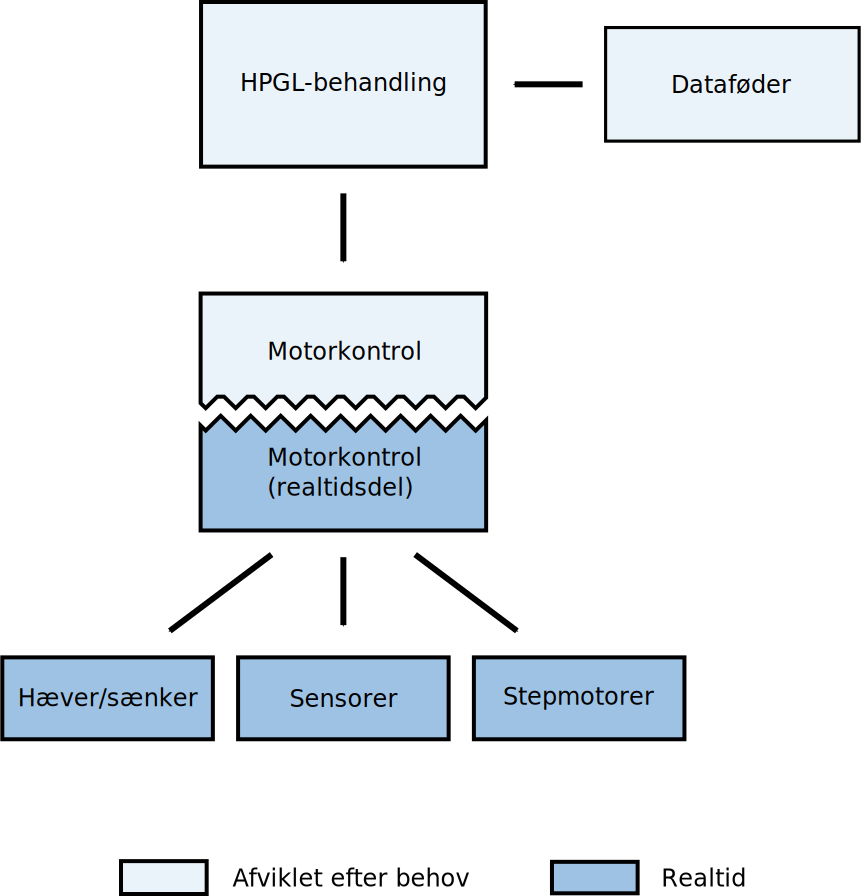
\includegraphics[width=.75\textwidth]{../brugere/kjaergaard/software-oversigt}
  \caption{Oversigt over softwaren. De lyseblå dele afvikles når der
    er tid til det. Når det er tid til at afvikle de mørkeblå områder,
    afbrydes afviklingen af de lyseblå.}
  \label{fig:software-oversigt}
\end{figure}


\section[Dataføder (med SPI og SD-/MMC-kort)]{Dataføder}

% Hvordan virker dataføderen (herunder buffer, spi og sd/mmc)?

Dataføderen leverer data til HPGL-motoren og håndterer de
underliggende moduler, der indeholder data.

Dataføderens skal
\begin{itemize} \firmlist
\item levere data til HPGL-motoren og sørge for at denne ikke løber
  tør for data\fixme{bliv enig om terminologi}
\item stille et ensartet API\footnote{Application Programming
    Interface, programmeringsbrugerflade; betegnelse for struktur og
    navngivning for funktioner, variable, strukturer, klasser
    etc. brugt til programudvikling.}\fixme{brug evt. wikis
    formulering af api} til rådighed uafhængig af underliggende modul,
  således at det overliggende modul er uafhængig af det modul, der
  indeholder data - se figur\vref{fig:datafeeder-uniform-api}
\item håndtere fejl for underliggende moduler
\end{itemize}

\mnote{
  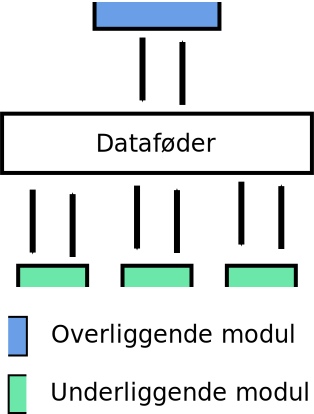
\includegraphics[width=\marginparwidth]{../brugere/kjaergaard/datafoeder-uniform-api}
  \captionof{figure}{Data\-føderen skal stille et ensartet API til
    rådighed.}
  \label{fig:datafeeder-uniform-api}
}

En oversigt over funktionsfordelingen\fixme{andet ordvalg} i
dataføreren\fixme{andet ordvalg} kan ses i
figur\vref{fig:software-spi-sd-oversigt}.

\begin{figure}[htbp]
  \centering
  \includegraphics[width=\textwidth]{../brugere/kjaergaard/datafeeder-oversigt}
  \caption{Diagram over funktionsfordeling i dataføderen.}
  \label{fig:software-spi-sd-oversigt}
\end{figure}

Kommunikationen med SD-kortet foregår gennem SPI'en\fixme{afsnit skal
  skrives færdig}. Et eksempel på en forespørgsel med tilhørende svar
kan ses i figur\vref{fig:software-spi-sd-handling}.

\begin{figure}[htbp]
  \centering
  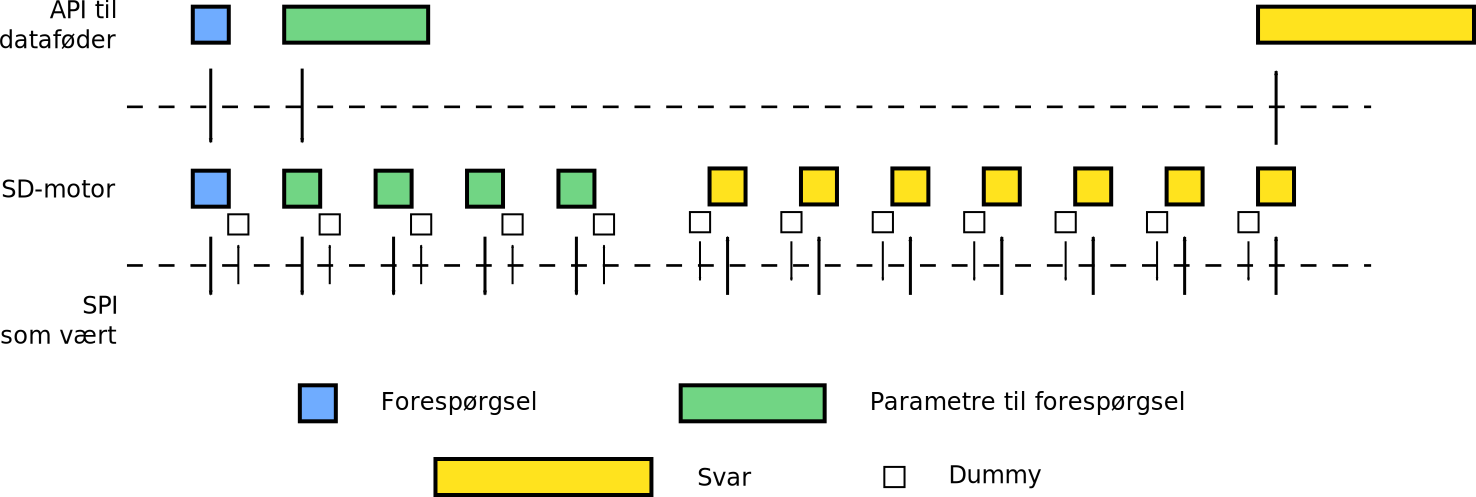
\includegraphics[width=\textwidth]{../brugere/kjaergaard/datafeeder-handling}
  \caption{Handlingdiagram ved kommunikation med SD-kortet.}
  \label{fig:software-spi-sd-handling}
\end{figure}


\section{HPGL-behandleren}

% Hvordan virker den del, der fortolker og behandler HPGL?
HPGL er et dataformat, som indeholder adskillige forskellige
instruktioner med forskellige parametre (se
afsnit\vref{sc:idn-ins-param}) . Vi benytter os ikke af samtlige
instruktioner, men blot et lille udvalg med udgangspunkt i vores
kravspecifikation.  I projektet anvender vi følgende instruktioner:

\begin{itemize} \firmlist
\item[\texttt{PU}/\texttt{PD}] Pen Up/Pen Down - bruges til at hæve og
  sænke pennen.
\item[\texttt{PA}/\texttt{PR}] Plot Absolut/Plot Relative - se
  afsnit\vref{sc:relativ-absolut}.
\item[\texttt{CI}] Plot Circle - se afsnit\vref{sc:matematik-cirkel}.
\end{itemize}

HPGL bruger oprindeligt bogstaver, tal og symboler (komma, punktum
osv.) til at identificere instruktioner, men som det fremgår af næste
afsnit, så anvender vi kun bogstaver i vores identifikation.

\subsection{Identifikation af instruktioner og parametre}
\label{sc:idn-ins-param}

% Her skriver vi hvordan vi identificerer instruktioner og parametre i
% datastrømmen

HPGL-behandleren identificerer instruktioner og parametre på
datastrømmen med en \textit{parser}. Databehandleren består af en
markør og pladsholdere til instruktioner og parametre.

Parseren er \textit{byte}-orienteret og kan kun se én byte ad gangen,
se figur\vref{fig:hpgl-parser-iden}. Afhængig af denne bytes værdi
gemmer parseren byten i en pladsholder og indlæser den næste byte for
at sætte kæden sammen til instruktioner eller parametre til
instruktioner.

% floaten ligger muligvis for lavt
\snote{
  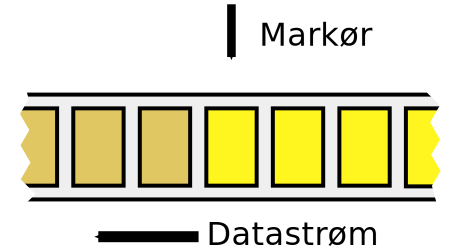
\includegraphics[width=\marginparwidth]{../brugere/kjaergaard/datafoeder}
  \captionof{figure}{Markøren på datastrømmen i HPGL-behandlerens
    identifikation af instruktioner på datastrømmen.}
  \label{fig:hpgl-parser-iden}
}

Hvis byten ikke har en værdi, parseren forstår, flyttes markøren
videre til næste byte, således at den byte, markøren peger på, ikke er
fortolket.

Hvis byten er et bogstav, peger markøren på første byte i en
instruktion. Den næste byte indlæses og de to byte sættes sammen til
en instruktion.

Hvis byten er et tal eller punktum (.), peger markøren på første byte
i en talparameter. Der indlæses og gemmes bytes indtil den indlæste
byte ikke er et tal eller punktum. Når den indlæste byte ikke er et
tal eller punktum, konverteres de indlæste bytes til et tal.

Se afviklingsdiagrammet for parseren i
figur\vref{fig:hpgl-parser-afvikling}. Parseren understøtter ikke
andre parametre end talparametre.

\begin{figure}[htbp]
  \centering
  \subfloat[Afviklingsdiagram for parserens instruktionsidentifikation.]{
    \includegraphics[width=.30\textwidth]{../brugere/kjaergaard/hpglparser-ins}
  }
  \qquad
  \subfloat[Afviklingsdiagram for parserens parameteridentifikation.]{
    \includegraphics[width=.60\textwidth]{../brugere/kjaergaard/hpglparser-param}
  }
  \caption{Afviklingsdiagrammer for HPGL-parseren.}
  \label{fig:hpgl-parser-afvikling}
\end{figure}


\subsection{Relative og absolutte koordinater samt grafikenheder}
\label{sc:relativ-absolut}

Indenfor HPGL bruger man relative og absolutte koordinater. Absolut
plotning indeholder to parametre, X og Y. X og Y er absolutte værdier,
altså kan de ikke være negative, som måles enten i en brugerdefineret
enhed eller grafik enheder (0,025mm). Absolut plot bruges, når man vil
flytte pennen til en bestemt koordinat set fra origo $(0, 0)$. Ligesom
med cirklen, så plottes kun en linie, når pennen er nede.

\mnote{
  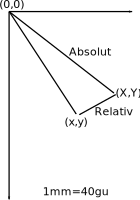
\includegraphics[width=\marginparwidth]{./img/relativ-absolut}
  \captionof{figure}{Eksempel på relativ og absolut linie}
  \label{fig:relativ-absolut}
}

Relativ plotning indeholder ligeledes to parametre, x og y. x og y er
relative værdier til den nuværende position, altså kan de godt være
negative. Relativ plotning måles ligesom absolut. Relativ plotning
bruges, når man vil lave serie af linier i række, da man her tager
udgangspunkt i den forrige linies
slutpunkt. Figur\vref{fig:relativ-absolut} viser et eksempel på
relative og absolutte linier.

\subsection{Behandling af cirkel}
\label{sc:matematik-cirkel}

Vi kender cirklens radius $r$, kordevinklen $c$ samt startkoordinater
$(x, y)$. Det første koordinat kan ud fra en hurtig analyse derfor let
findes:
\begin{align*}
P_0(x, y)=(r, 0)
\end{align*}

\mnote{
  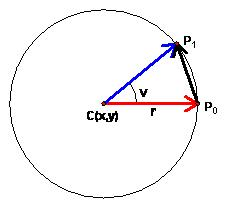
\includegraphics[width=\marginparwidth]{./img/cirkel}
  \captionof{figure}{Cirkel}
  \label{fig:cirkel-tegning}
}

Dette er tilfældet, da vinklen $w$ er $0\degree$.

Næste koordinat ligger i en vinkel $w$, som svarer til kordevinklen
$c$, altså har vi lagt en kordevinkel til de $0\degree$. Ved brug af
cosinus og sinus samt radius $r$ kan vi bestemme det næste koordinat:
\begin{align}
P_1(x, y)&=(\cos(w)\times r, \sin(w)\times r) \Rightarrow \nonumber \\
P_1(x, y)&=(\cos(c)\times r, \sin(c)\times r) \label{eq:8.1}
\end{align}
 
Denne formel kommer ud fra grundlæggende trigonometri:
\begin{align*}
\cos(v) &= \frac{x}{r} \Rightarrow x = \cos(v)\times r \\
\sin(v) &= \frac{y}{r} \Rightarrow y = \sin(v)\times r
\end{align*}
 
Formlen \vref{eq:8.1} kan omskrives, så den gælder et vilkårligt punkt
på cirkelperiferien:\fixme{denne henvisning er usikker}
\begin{align}
P_n(x, y)=(\cos(n\times c)\times r, \sin(n\times c)\times r)
\end{align}

Vi betragter en cirkel med en radius på 5cm og en kordevinkel på
$3\degree$. Første koordinat er således:
\begin{align*}
P_0(x, y)&=(\cos(0\times 3\degree)\times 5 , \sin(0\times 3\degree)\times 5)=(5, 0) \\
\end{align*}

Vi ser, at dette passer i overensstemmelse med første
udsagn. Vha. ovenstående formel kan vi blot lægge en til $n$ hver gang
funktionen er udført. Dette skal den blive ved med indtil vinkel
overskrider $360\degree$.


Der opstår dog et problem, hvis vinklen ikke går op i $360\degree$,
såsom vinklen $7\degree$. $51\times 7\degree = 357\degree \Rightarrow
rest = 3\degree$. Overskrider vinklen de $360\degree$, har vi to
muligheder:
\begin{itemize} \firmlist
\item Funktionen afsluttes uden at slutte cirklen
\item Funktionen ændres, så optegningen fortsætter til udgangspunktet $P_0$
\end{itemize}
Det skal også nævnes, at HPGL tegner uanset om pennen er oppe eller
nede, hvilket betyder, at vi skal bruge en funktion til at hæve og
sænke pennen. HPGL sender "PU" (Pen Up), når pennen skal være
oppe. Tilsvarende sender den en "PD" (Pen Down), når der skal
tegnes. Pennen starter i cirklens centrum. Vi skal derfor sikre os, at
pennen er hævet før den går til første punkt $P_0$. Herefter bruger vi
den generelle funktion til at bestemme x,y-koordinaterne. Efter hver
udført funktion lægges en ekstra kordevinkel til vinklen indtil
vinklen $w$ er større eller lig $360\degree$. Herefter hæves pennen og
flyttes tilbage til cirklens centrum. Afviklingsdiagrammet viser denne
proces (se figur\vref{fig:hpgl-cirkel-afvikling}).

\begin{figure}[htbp]
  \centering
  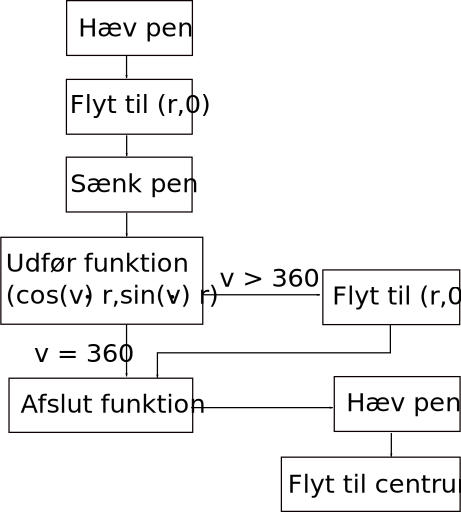
\includegraphics[width=0.5\textwidth]{./img/afviklingsdiagram-cirkel}
  \caption{Afviklingsdiagram for cirkelplot}
  \label{fig:hpgl-cirkel-afvikling}
\end{figure}


\section[Motorkontrol (med buffer)]{Motorkontrol}

% Hvordan er motorkontrollen implementeret? Beskriv implementeringen
% kort.



\begin{figure}[htbp]
  \centering
  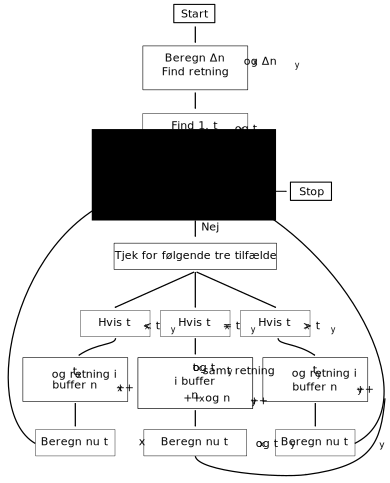
\includegraphics[width=.75\textwidth]{./img/la-behandling}
  \caption{Afviklingsdiagram over afvikling af LA-instruktionen.}
  \label{fig:la-behandling}
\end{figure}


\section{Stepmotorstyring}

% Hvordan styres stepmotorerne? Superkort. Hvordan ser softwaren der
% styrer dem ud?


\section{Sensorer og løfter/sænker}


%%% Local Variables: 
%%% mode: latex
%%% TeX-master: "../master"
%%% End: 